\documentclass[11pt]{article}

% ============================================================
%  AI Applications in Research: The Claude Code Workflow
%  A conceptual summary synthesised from Scott Cunningham's
%  "Scott's Mixtape" Claude Code series (Dec 2025 - Aug 2026).
% ============================================================

\usepackage[margin=1in]{geometry}
\usepackage{amsmath}
\usepackage{amssymb}
\usepackage{enumitem}
\usepackage{titlesec}
\usepackage{xcolor}
\usepackage{tikz}
\usepackage[colorlinks=true,linkcolor=black,urlcolor=blue!60!black]{hyperref}

\definecolor{accent}{RGB}{31,73,125}
\titleformat{\section}{\Large\bfseries\color{accent}}{\thesection}{0.75em}{}
\titleformat{\subsection}{\large\bfseries\color{accent!85!black}}{\thesubsection}{0.6em}{}

\newcommand{\keyword}[1]{\textbf{\color{accent}#1}}

\title{\vspace{-1.5em}\textbf{AI Applications in Research}\\[0.3em]
\large A Conceptual Summary of Agentic Empirical Workflows,\\ with a Focus on Claude Code}
\author{Compiled from Scott Cunningham's \emph{Scott's Mixtape} Claude Code series}
\date{19 August 2026}

\begin{document}
\maketitle

\begin{abstract}
\noindent This document summarises the main concepts that have emerged around the
use of AI agents---and Claude Code in particular---in quantitative empirical
research. It is synthesised from Scott Cunningham's ongoing ``Claude Code for
quantitative social scientists'' series. The central claim is that AI agents have
made the \emph{production} of research nearly costless, which shifts the binding
constraint of the research enterprise onto \emph{verification} and \emph{human
understanding}. The document organises the key ideas into an economic framing (the
collapse of the marginal cost of research), an epistemological framing (the
production--verification--understanding triangle), and a practical framing (agentic
workflows, checklists, hooks, and skills as implemented in Claude Code).
\end{abstract}

\tableofcontents
\vspace{1em}

% ------------------------------------------------------------
\section{The New Capability: ``3-D Printing'' a Research Paper}
% ------------------------------------------------------------

The starting observation is that modern coding agents (Claude Code, Codex, and
comparable tools) can now carry an empirical research project from a blank prompt
to a submittable manuscript essentially end-to-end. Given only a high-level
instruction, an agent can:

\begin{itemize}[leftmargin=1.4em]
  \item choose a research question and an identification strategy;
  \item locate the relevant datasets online and download them locally;
  \item select an estimator, write replicable code (in any language), and organise
        it in a local directory;
  \item produce the exhibits---tables, figures, and a battery of robustness checks;
  \item write the full manuscript (references, appendices, and all) in roughly the
        time it takes to read this page.
\end{itemize}

Cunningham calls this \keyword{``3-D printing a research paper.''} The Social
Catalyst Lab's autonomous program-evaluation project---in which agents endogenously
produced roughly one thousand difference-in-differences / instrumental-variables
``program evaluation'' papers under human prompting---demonstrates that this is no
longer a conjecture. Agents \emph{can} autonomously and endogenously produce
empirical research.

\subsection{But autonomy is not full self-driving}
The crucial qualification is that raw \emph{production} capability does not equal
trustworthy research. Cunningham's metaphor: today's agent is less a fully
autonomous vehicle than a car with \keyword{lane-keeping and cruise control}---it
holds a lane and maintains speed, but a human must remain at the wheel. The reason
is that production is only one of three things a credible research output must
satisfy.

% ------------------------------------------------------------
\section{The Economic Framing: The Collapsing Marginal Cost of Research}
% ------------------------------------------------------------

Before AI agents, the quantity of research a person produced was pinned down by the
marginal cost of production, $MC_b$, which was fixed by scarce human time and skill.
Research was produced up to the point where marginal benefit equalled that marginal
cost.

AI agents drive the marginal cost of production down to some small
$\widehat{MC}_{AI} = \varepsilon \approx 0$. Two consequences follow:

\begin{enumerate}[leftmargin=1.4em]
  \item \keyword{More research is produced}, moving output from $Q^*_b$ to
        $Q^*_{AI}$ (with the elasticity set by the shape of the demand curve).
  \item \keyword{New surpluses appear.} The old work is now done with far fewer
        time inputs (a surplus gain on inherited output), and additional output
        generates further surplus.
\end{enumerate}

\begin{center}
\begin{tikzpicture}[scale=0.95]
  % axes
  \draw[->] (0,0) -- (7,0) node[right] {\small Quantity of research $Q$};
  \draw[->] (0,0) -- (0,5) node[above] {\small Marginal value / cost};
  % demand curve
  \draw[thick,accent] (0.3,4.6) -- (6.6,0.4) node[below right] {\small Demand};
  % old MC
  \draw[dashed] (0,3.0) node[left] {\small $MC_b$} -- (6.5,3.0);
  % new MC
  \draw[dashed] (0,0.6) node[left] {\small $\widehat{MC}_{AI}$} -- (6.5,0.6);
  % old quantity
  \draw[dotted] (2.35,0) node[below] {\small $Q^*_b$} -- (2.35,3.0);
  % new quantity
  \draw[dotted] (5.75,0) node[below] {\small $Q^*_{AI}$} -- (5.75,0.6);
\end{tikzpicture}
\end{center}

\subsection{The hidden cost: understanding was a by-product of production}
The subtle point is that, under the old human mode of production, \emph{understanding
was produced automatically as a by-product of doing the work}. To make a result you
generally had to understand it first, and you understood it further simply by having
made it---a kind of ``squatter's right'' of comprehension over one's own output.

When the agent does the producing, that automatic understanding no longer arrives for
free. The researcher becomes like a lab manager or principal who must trust an agent
(the ``RA'') they did not supervise closely. This raises a \keyword{principal--agent
problem}: we trust the work was done well, but the agent is not accountable, our own
skills may atrophy, and we may lose the ability to judge what ``done well'' even means.
The saved time can, in principle, be reinvested into rebuilding that understanding---but
only deliberately, never automatically.

% ------------------------------------------------------------
\section{The Epistemological Framing: Production, Verification, Understanding}
% ------------------------------------------------------------

The organising idea of the series is that credible research with agents must pass
through \keyword{three distinct ``doors''}:

\begin{center}
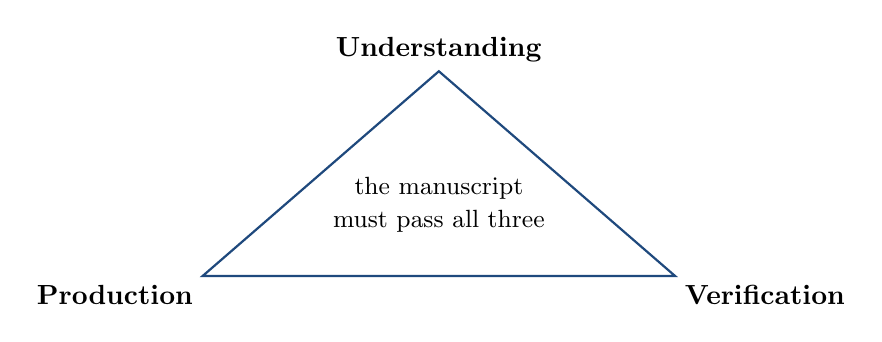
\begin{tikzpicture}[scale=1.0]
  \coordinate (P) at (0,0);
  \coordinate (V) at (6,0);
  \coordinate (U) at (3,2.6);
  \draw[thick,accent] (P) -- (V) -- (U) -- cycle;
  \node[below left]  at (P) {\textbf{Production}};
  \node[below right] at (V) {\textbf{Verification}};
  \node[above]       at (U) {\textbf{Understanding}};
  \node[align=center] at (3,0.9) {\small the manuscript\\ \small must pass all three};
\end{tikzpicture}
\end{center}

\begin{description}[leftmargin=1.5em,style=nextline]
  \item[Production] Generating the analysis and the manuscript. This is what agents
        already do well and autonomously.
  \item[Verification] Confirming the output is accurate. Replicating code across
        languages and checking that every exhibit was generated by stored code are
        \emph{necessary but not sufficient}. True verification is endogenous to a
        \emph{pre-registered target estimand}: it confirms that what we set out to
        do was in fact done---\emph{and that what should not have been done was not
        done}. Agents cannot check the latter, because ``things that should not have
        happened'' leave nothing to point at. A documented failure mode is
        \keyword{endogenous specification sorting}: agents drift into model
        specifications in response to true statements about the project, not just
        explicit instructions.
  \item[Understanding] The human must retain full, accurate comprehension of what was
        done, by whom, and what was found. The analogy is the \keyword{CEO} who need
        not write the code but must nonetheless know---approximately but truthfully---that
        each task was done, by whom, and with what result.
\end{description}

\subsection{Zero errors as a constraint, not an objective}
Verification and understanding are imposed as a hard constraint: \keyword{zero
errors}. This is deliberately \emph{not} error \emph{minimisation}, which would
license an ``optimal'' positive number of mistakes. Instead, ``zero errors'' enters
as a binding constraint in the Lagrangean of producing the manuscript, which must
simultaneously satisfy production, verification, and understanding. Echoing the old
IBM maxim: \emph{a machine cannot be held accountable, therefore a machine must not
be left to make the decision}---agents either help us understand what they did, or we
do not use them.

% ------------------------------------------------------------
\section{The Practical Framing: Harnesses, Checklists, Hooks, and Skills}
% ------------------------------------------------------------

The workflow answer to the verification/understanding constraint is to wrap the agent
in structure rather than to trust free-form autonomy.

\subsection{The checklist / ``harness''}
Cunningham centres his method on a method-specific \keyword{harness}---currently a
difference-in-differences harness, deliberately kept narrow so it can be evaluated
and perfected before generalising (it plausibly extends to synthetic control,
unconfoundedness, and other designs). The concept is drawn from Atul Gawande's
\emph{The Checklist Manifesto}: high-stakes work fails because people skip critical
steps, and---counter-intuitively---\emph{experts} skip more steps than beginners
(Kahneman's fast ``System 1'' thinking). A checklist forces every project through the
three doors. The harness is intentionally \emph{visual}, mapping the analytic pipeline
into cards and exhibits.

\subsection{The ``bite'' stage: what \emph{not} to automate}
An illustrative checklist item is the \keyword{``bite''} stage: documenting the very
first real-world response to an intervention (e.g., for a gun law, the movement of
guns; for a minimum-wage change, where the wage floor actually binds), exhaustively,
across the two dimensions of \keyword{space} (heat maps) and \keyword{time} (time-series
aggregations, including comparison groups).

Although an agent \emph{can} draw the maps, write the code, and download the data,
Cunningham argues the bite stage should \emph{not} be fully automated, because it is
where the project is conceived and where the researcher discerns the
\keyword{treatment assignment mechanism}---the crux of design-based (as opposed to
parametric) causal inference. The main mechanisms and their matching designs:

\begin{itemize}[leftmargin=1.4em]
  \item \textbf{Human rationality / essential heterogeneity} (endogenous, optimising
        choice; Heckman's Roy model, Rubin's ``perfect doctor'')---the case that makes
        naive causal inference nearly impossible, as LaLonde (1986) showed.
  \item \textbf{Instruments} $\Rightarrow$ instrumental variables (randomised
        assignment via the instrument; requires the exclusion restriction).
  \item \textbf{Randomised treatment} $\Rightarrow$ RCTs.
  \item \textbf{Running variables} $\Rightarrow$ regression discontinuity.
\end{itemize}

The lesson: automate exhibit and manuscript \emph{production} (via hooks and skills),
but keep the human firmly in charge of the conceptual, design-defining detective work.

\subsection{Hooks and skills}
The concrete mechanisms Claude Code offers for encoding this discipline:
\begin{itemize}[leftmargin=1.4em]
  \item \keyword{Hooks} --- automation wired into each checklist step (e.g., figure
        and table production, assembling exhibits into a deck or manuscript), ideally
        \emph{specific} to each stage rather than abstract and universal.
  \item \keyword{Skills} --- reusable, invokable routines. Two examples aimed at
        \emph{understanding} rather than output:
        \begin{itemize}[leftmargin=1.2em]
          \item an \keyword{interview} skill that extracts the researcher's beliefs
                (which covariates, what target parameter) when they are uncertain but
                suspect they know;
          \item a \keyword{/quiz} skill inspired by corporate compliance training:
                Claude Code generates teaching slides on the project, then asks the
                researcher multiple-choice questions one at a time---continuously
                rebuilding human understanding on top of verification.
        \end{itemize}
\end{itemize}

% ------------------------------------------------------------
\section{Synthesis: What the Bottleneck Actually Is}
% ------------------------------------------------------------

Two slogans frame the shift. Geoffrey Litt's ``\emph{Understanding is the new
bottleneck}'' (surfaced by Paul Goldsmith-Pinkham) complements Cunningham's own
``\emph{Verification is the new bottleneck}.'' Both express the same reallocation:
once production is nearly free, the scarce, value-determining activities are
confirming that the output is correct and ensuring a human genuinely comprehends it.

\begin{center}
\fbox{\begin{minipage}{0.9\textwidth}
\centering
\textbf{Core takeaway.} AI agents have collapsed the marginal cost of
\emph{producing} research toward zero. The binding constraints have moved to
\emph{verification} and \emph{understanding}. Good agentic research practice
therefore means deliberately re-investing the freed time into structure---checklists
and harnesses, stage-specific hooks, and understanding-oriented skills (interviews,
quizzes)---so that the human remains the accountable ``CEO'' of a process held to a
\emph{zero-errors} constraint.
\end{minipage}}
\end{center}

% ------------------------------------------------------------
\section*{Sources and Further Reading}
\addcontentsline{toc}{section}{Sources and Further Reading}
% ------------------------------------------------------------

\begin{itemize}[leftmargin=1.4em]
  \item Scott Cunningham, \emph{Scott's Mixtape Substack} --- the ``Claude Code for
        quantitative social scientists'' series (Dec 2025--Aug 2026), especially:
        ``Which stages of research production should we let AI Agents loose''
        (14 Aug 2026); ``How to improve understanding with Claude Code'' (7 Aug 2026);
        ``My strategy for talks on agents for research'' (10 Aug 2026).
        \url{https://causalinf.substack.com/s/claude-code}
  \item Geoffrey Litt, ``Understanding is the new bottleneck.''
  \item Atul Gawande, \emph{The Checklist Manifesto}.
  \item Daniel Kahneman, \emph{Thinking, Fast and Slow}.
  \item R.~LaLonde (1986); Imbens \& Angrist (1994, LATE); Imbens \& Lemieux
        (RDD: A Guide to Practice); Rubin, ``Design Trumps Analysis.''
  \item Scott Cunningham, \emph{Causal Inference: The Remix} (Yale University Press,
        2026) --- free online edition. \url{https://causalinf.substack.com/}
\end{itemize}

\end{document}
